
\section{Introduction}

The release of the RefSeq v1.0 genome assembly of bread wheat cultivar Chinese
Spring~\citep{IWGSC2018} provided the first detailed map of the 16Gb genome bringing wheat genomic
resources closer to the standard enjoyed in rice and maize. 
%
Already, international efforts are in the process of assembling more than ten elite wheat varieties
to a similar standard. 
%
Within five years we can expect hundreds of high quality wheat genomes to be available. 
%
The challenge that remains is to connect these new resources to the wealth of research carried out
in the past few decades, and make this information accessible to researchers and breeders who may
lack the required bioinformatics skill-set.
%
Existing tools such as cMap~\citep{fang2003cmap} or genome
browsers~\citep{Stein2013GBrowse,Buels2016JBrowse} allow the visualisation of genetic maps and genome
assemblies, respectively, but are separate tools. Hence one cannot view a genetic map alongside a
physical genome sequence, for example. 
%
Wheat-focused databases such as GrainGenes and T3~\citep{Blake2016T3} provide a wealth of legacy
data but can be difficult to interface with. 
%
Pretzel aims to provide a framework that combines curated data stored in a back-end with a
modern front-end graphical user interface for visualisation and analysis via a web browser. 
%
\begin{figure*}
\centering
  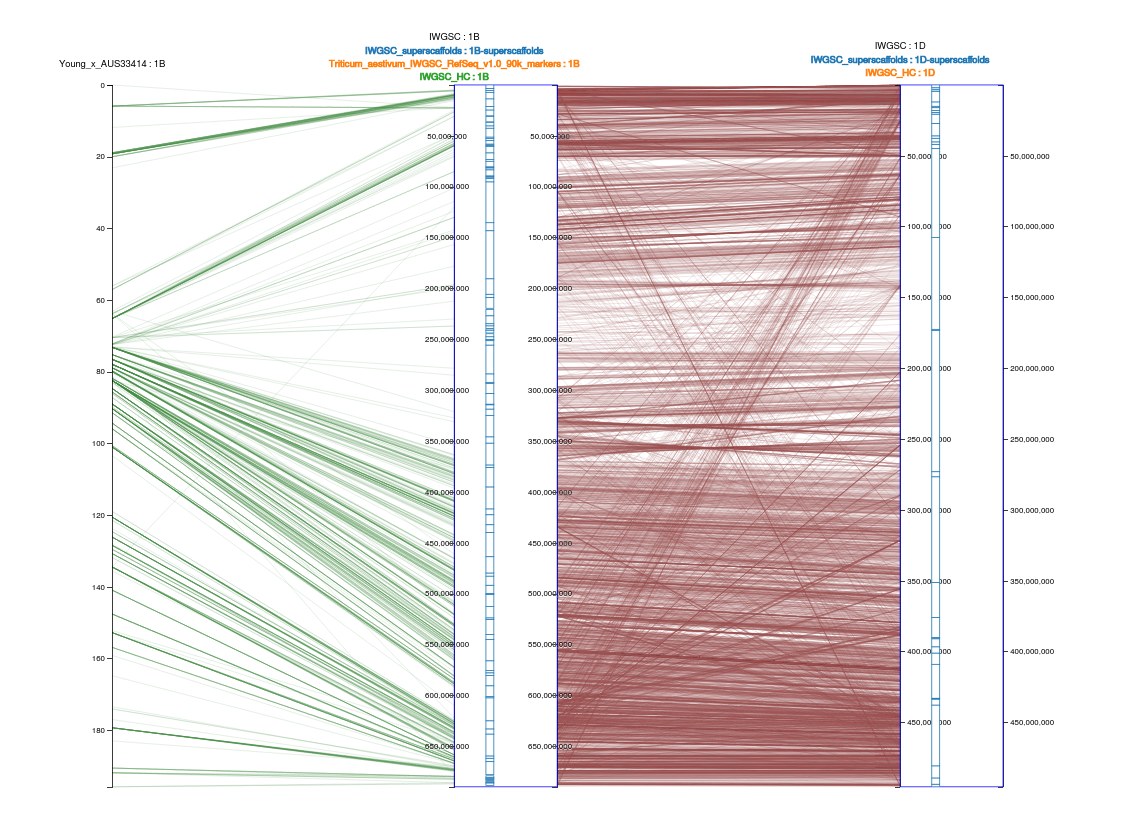
\includegraphics[width=\textwidth]{pretzel.png}
\caption{
  Pretzel alignment showing a 90k genetic map on the far left against the IWGSC RefSeq v1.0 chromosome 1B pseudomolecule in the centre, 
  with chromosome 1D on the far right. 
  Green lines between features indicate direct, e.g. marker-based links. 
  Red lines indicate links via alias which can be definded e.g. based on sequence similarity. 
  The two pseudomolecules have their scaffold arrangement displayed in blue, alongside their axes.
}
\label{fig:01}
\end{figure*}
%
%\begin{methods}
\section{Methods}

Pretzel is built on several JavaScript frameworks: the front-end combines Ember.js with D3.js
  for real-time visualisation; the back-end is in Loopback.js connecting to a MongoDB database. 
%
The user interacts with Pretzel via a web page served by the front-end. 
%
The data model has been designed to be as general as possible while still enabling the richness of
  data to be captured. 
%
  The highest level data structure is a \textit{dataset}, which contains one or more \textit{blocks}.
%
For example, a dataset may describe a genetic map, where the blocks are individual linkage groups. 
%
  Within each block are a set of \textit{features} which are defined as intervals (possibly of zero length,
  which would define a single position) within the block. 
%
For example, a feature could be a molecular marker in a linkage group, or the position of a gene in
  a physical chromosome. 
%
Using only these three concepts, a large number of concepts can be represented: a quantitative trait locus
  (QTL) is simply an interval \textit{feature} within a linkage group \textit{block}; whereas pseudomolecule structure can be described by a
  set of intervals denoting scaffold start/end positions \textit{features} within a chromosome \textit{block}. 
%
As there are often multiple alternative names for molecular markers we created a fourth concept \textit{alias}. 
\textit{Alias} enables features with different names to be considered as the same and therefore linked when drawing alignments. 
%
At present this general concept allows the association of syntenic genes between genomes and the direct comparison of genetic maps
  based on different marker systems/types through alias by reference position.

Data uploaded is simple and can be achieved through the web interface in CSV or JSON format (the native data structure in
  JavaScript); or uploaded via command line in JSON format directly to the back-end. 
%
Data sets can be uploaded in whole or in part, or as they are generated, providing flexibility and allowing users to add data in real time.
%
Upon upload, data is visible by that user only, unless they explicitly make it available to other users. 
%
In addition, we have created a pipeline, 
  \href{https://github.com/plantinformatics/pretzel-input-generator}{https://github.com/plantinformatics/pretzel-input-generator}), 
  to generate Pretzel-ready data
  from standard genome assembly formats in an automated way. This pipeline has been used to make
  available a set of publicly available genomes so users can quickly set up a Pretzel server
  populated with real data.

A common goal in wheat genetic studies is to fine map a QTL to discover the underlying gene. This generally requires the translation of the
  QTL region from genetic map space to physical genome space. Once this is achieved one of the most common questions asked in wheat research 
  is what genes underlie a QTL interval defined in a genetic mapping experiment. 
%
With Pretzel, users with no bioinformatics training can quickly project their genetic map interval
  onto physical sequence and extract the genes in the target region for downstream analysis. 
%
An additional challenge when fine mapping an interval is potential mis-assembly in the region
  of interest. Figure~\ref{fig:01} shows a genetic map aligned to a physical chromosome, as well as
  two syntenic chromosomes (chromosomes 1B and 1D) aligned via their syntenic genes (shown in red). 
%
By comparing the co-linearity of genes between sub-genomes, potential assembly problems can be
  flagged by noting when abrupt changes in co-linearity occur at scaffold break points. 
%
In this way, advanced curation of pseudomolecule structure can be achieved on any number of genomes.

The technology stack Pretzel is built on is lightweight and a user with the necessary dependencies
can clone, build and run the Pretzel code within minutes with a few simple commands. 
%
If run on an internet-facing machine, external users can then connect to the server.
%
To make the installation process even easier, we provide Docker container images on Docker Hub
(\href{https://hub.docker.com/r/plantinformaticscollaboration/pretzel/}{\nolinkurl{https://hub.docker.com/r/plantinformaticscollaboration/pretzel/}}).
%\end{methods}

\section{Conclusion}

We have developed a web-based visualisation and analysis tool that solves many challenges posed today in wheat research. 
%
Its development is ongoing and we believe the volume of data that will be publicly available in the next few years will only increase its utility and relevance.

\section*{Acknowledgements}

Blah di blah.

\section*{Funding}

This work has been supported by the Grains Research and Development Corporation project DAV00127.\vspace*{-12pt}

\bibliographystyle{natbib}

\bibliography{references}
